\qns{Practice with $\bm{j_\nu}$, $\bm{\alpha_\nu}$, $\bm{S_\nu}$, $\bm{I_\nu}$}

\begin{enumerate}
\qitem{
	\begin{itemize}
		\item $n_\text{gas} \sim 10\si{\centi\meter}^{-3}$
		\item $\rho_\text{dust}/\rho_\text{gas} = 0.01$
		\item $r_\text{grain} = 0.1\si{\micro\meter} = 10^{-5}\si{\centi\meter}$
		\item $\rho_\text{grain} \sim 3\frac{\si{\gram}}{\si{\centi\meter}^3}$
	\end{itemize}}

\work{
	\begin{multicols}{2}
		\raggedcolumns
		\begin{align*}
			\rho_\text{gas} &= \frac{2}{N_0}n_\text{gas}\\
				&\approx \frac{1}{3}\left(10^{-22}\right) \frac{\si{\gram}}{\si{\centi\meter^3}}\\
			\rho_\text{dust} &= \frac{\rho_\text{gas}}{100}\\
				&\approx \frac{1}{3}(10^{-24}) \frac{\si{\gram}}{\si{\centi\meter^3}}
		\end{align*}
		\vfill\columnbreak
		\begin{align*}
			n_\text{dust} &= \frac{\rho_\text{dust}}{m_\text{grain}}\\
				&= \frac{\rho_\text{dust}}{V_\text{grain}\rho_\text{grain}}\\
				&= \frac{\rho_\text{dist}}{\frac{4}{3}\pi r_\text{grain}^3 \rho_\text{grain}}\\
				&\approx \frac{1}{12\pi}(10^{-9}) \frac{\text{particles}}{\si{\centi\meter^3}}
		\end{align*}
	\end{multicols}}

\ans{
	\begin{align*}
		n_\text{dust} &\approx \frac{1}{12\pi}(10^{-9}) \frac{\text{particles}}{\si{\centi\meter^3}}\\
			&\approx 2.65(10^{-11})\frac{\text{particles}}{\si{\centi\meter^3}}
	\end{align*}}

\newpage
\qitem{
	\begin{itemize}
		\item $I_{\nu 0} = 3(10^{-3}) \frac{\text{erg}}{\si{\second\cdot\hertz\cdot\steradian\cdot\centi\meter^2}}$
		\item $\nu = 1\si{\tera\hertz}$
	\end{itemize}}

\work{
	\begin{align*}
		\alpha_\nu &= n_\text{dust}\sigma_\text{grain}\\
			&= n_\text{dust}\cdot \pi r_\text{grain}^2\\
			&\approx \frac{1}{12}(10^{-19}) \frac{1}{\si{\centi\meter}}
	\end{align*}}

\ans{
	\centering
	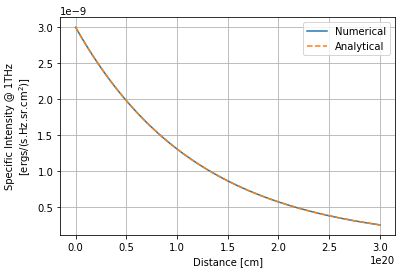
\includegraphics[width=0.7\textwidth]{./questions/q_dust_extinction_emission_figs/extinction.png}}

\newpage
\qitem{
	\begin{itemize}
		\item $T = 50\si{\kelvin}$
	\end{itemize}}

\work{
	\begin{align*}
		B_\nu(\nu,T) &= \frac{2h\nu^3}{c^2}\frac{1}{e^{\frac{h\nu}{k_BT}} - 1}\\
			&\approx 9.6(10^{-12}) \frac{\text{erg}}{\si{\second\cdot\centi\meter^2\cdot\steradian\cdot\hertz}}\\
		j_\nu &= B_\nu \sigma_\text{grain} n_\text{dust}\\
			&\approx 8(10^{-32}) \frac{\text{erg}}{\si{\second\cdot\centi\meter^3\cdot\steradian\cdot\hertz}}
	\end{align*}}

\ans{
	\centering
	$$I_{\nu,\text{medium}}(s) = \frac{j_\nu}{\alpha_\nu}\left(1-e^{-\alpha_\nu s}\right)$$
	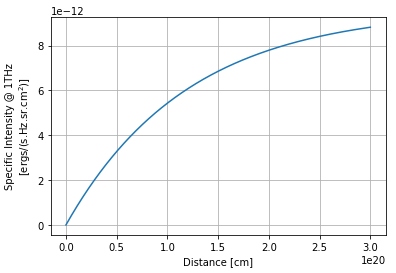
\includegraphics[width=0.7\textwidth]{./questions/q_dust_extinction_emission_figs/emission.png}}

\newpage
\qitem{}

\work{
	Combining the answers from before}

\ans{
	\centering
	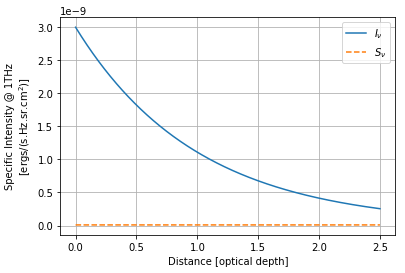
\includegraphics[width=0.7\textwidth]{./questions/q_dust_extinction_emission_figs/emission_extinction_tau.png}}

\end{enumerate}